\chapter{Results}
\label{cha:results}
% This chapter should display the results of your experiments. It should be entirely
% factual, so leave the discussion you draw from it for the Discussion chapter.
%
% You may choose to structure your thesis slightly differently, but the overall 
% approach should be the same.
%
% 1. By now you should have already described your methodology and  evaluation 
%    procedures. There is no reason to discuss these in the results.
% 2. Do not include raw data in the results chapter, leave it for the appendix 
%    or simply don't include it. If you don't think people will refer to it it's
%    probably not worth including.
% 3. Display your results in an informative way. Charts, tables, summaries, etc.
%
% If your results form a complete chapter you can use the conclusion section to
% state how the results answer your hypothesis. If you don't have a spearate
% conclusion chapter make sure you answer the hypothesis as you go. The reader
% should have answers to these before the Discussion.

The problem at hand along with the methodology employed to produce the solution are now well defined. Paired with an understanding of important previous works in this area and the technologies available, the design of each of the components may be given consideration. This chapter will present the designs of the required additions to the Gene-Plex Extractor, as were defined in Section \ref{sec:intro_scope}, Scope. This will include relevant results from stages of the design process, the conducted simulations along with validations and verifications via experimental methods. Through the sections below, the reader will be familiar with the design of each of the components along with the resulting performance of the realised and implemented component.\\

\section{Processor Module}

\subsection{Hardware}

\subsubsection{Thermal Isolation}

The first consideration given to the design of the physical Processor Module was the thermal isolation of the heated and non-heated volumes. While there is no requirement stipulating that only tubes 2 and 3 may be heated, it was deemed  thermally inefficient to heat the entire module. Such a design would also decrease the performance of the controller due to the larger mass to be heated. Therefore, the module was split into two regions, refereed to as the Thermal Region and the Carrier. While the method of isolation needed to be effective to create a stable and controllable thermal system, a number of other design considerations were present:
\begin{enumerate}
	\item[Manufacturability] The design of the thermal isolation method needed to consider the available manufacturing methods and their capabilities. For example, concept A shown in Figure \ref{fig:splitconcepts}, utilized a simple "trench" to create an air gap between the heated and non-heated regions of a single block of aluminium. While this concept satisfied the serviceability and cost objectives, there were a number of physical constraints preventing it from being feasible. Due to the geometry of the cassettes, the trench width was limited to 3mm across. At this size, the maximum depth at which the tooling could cut was stated to be 30mm \cite{Sorenson}. At this depth, not only would a large area of material still connect the two regions, but the cost of machining would be high.
	\item[Serviceability] When considering the serviceability of the product, two main aspects were key. This includes the initial assembly of the device after manufacture along with the periodic maintenance during its operating life. The resulting design must ensure manual assembly is practical and that the replacement of components, such as sensors or heating hardware is considered. 
	\item[Cost] Given that a total of 3 Processor Modules are required for each Gene-Plex Extractor, the designs selected must be cost effective. while a number of high cost manufacturing methods or materials may have met the needs of the thermal isolation requirement, the cumulative cost required led to a need for alternative concepts to be generated.
\end{enumerate}	

With these factors in mind, four main concepts were generated with the goal of insulating the thermally controlled region of the Processor Module from the non-heated portion in mind. These concepts are displayed in Figure \ref{fig:splitconcepts}.\\

\begin{figure}[!htb]
	\centering
	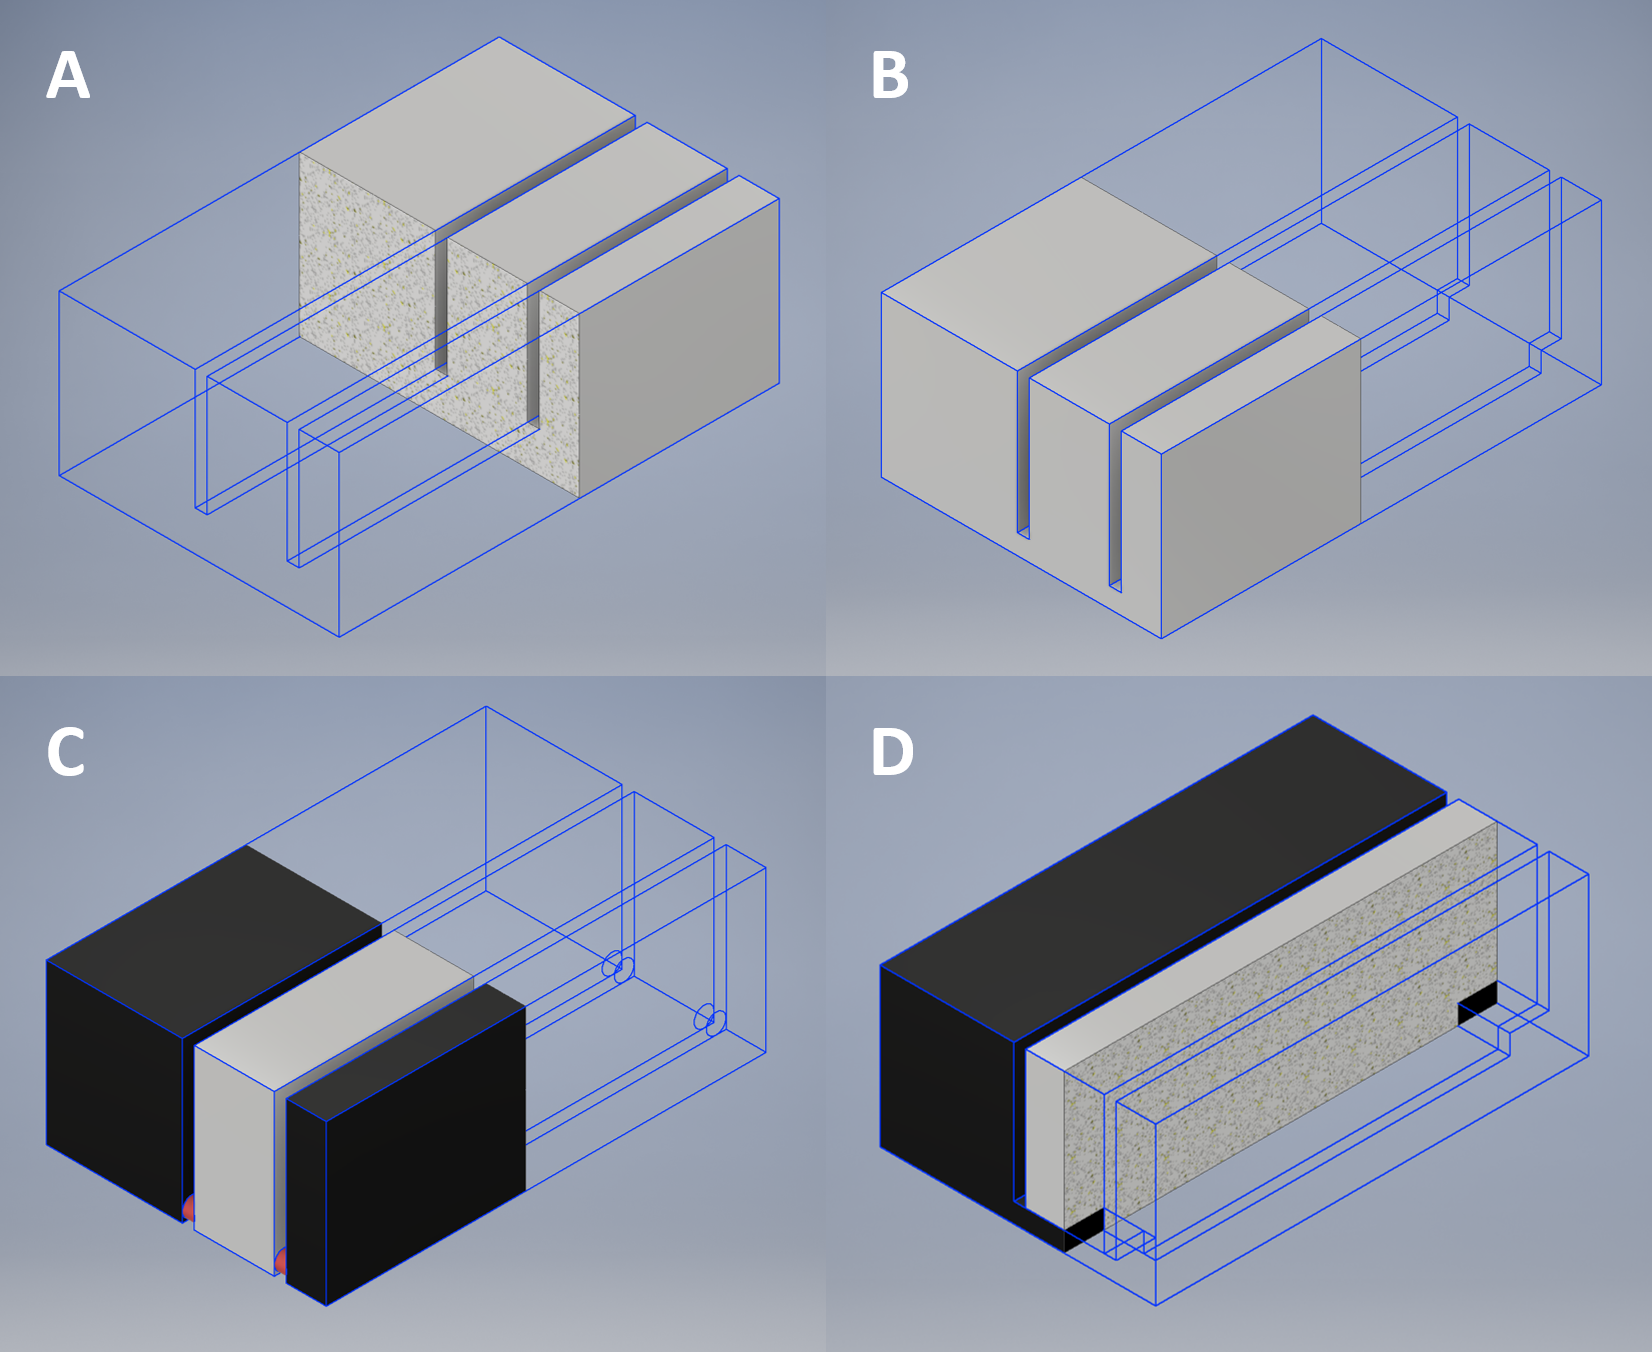
\includegraphics[width = \textwidth]{splitconcepts.png}
	\caption[Thermal Insulation Concepts.]{CAD representations of the thermal insulation concepts.}
	\label{fig:splitconcepts}
\end{figure}ˆ 
\FloatBarrier

Concept A features a groove machined into a solid billet of Aluminium, forming an air gap between the two regions. This concept has the advantage of simplicity, aiding with manufacture and serviceability. It's use of a single piece of material is also cost effective. It however had two main drawbacks. With the groove limited to a maximum of 3mm width and therefore 30mm deep, there is a large portion of material remaining which joins the two regions, leading to an undesirable level of heat transfer. Furthermore, the tooling costs involved with manufacturing this concept with the high aspect ration groove are significantly higher than with traditional machining operations. For these reasons, this concept required further development.\\

Concept B furthered the ideal behind Concept A by improving on some of its flaws, namely the transfer of heat. This was achieved by including further machining operations on the bottom face of the block. Therefore, the groove depth could be through the thickness of the block, apart from the small connecting regions on the outer edges of each groove. This simple change allowed the connecting area of material to be reduced to only 10\% of that of Concept A. Despite these improvements, the extra operations still require that small sections be machined at the same 30mm depth with the 3mm tool bit. Avoiding this is possible by performing machining operations on all four faces as opposed to only the top and bottom, however this will still carry added cost. Further to this, the homogeneous material and solid connection would allow for a more rapid heat transfer than was desirable. While aluminium is required for the Thermal Region due to its high level of heat transfer, this will result in large energy losses to the Carrier. It was therefore decided that the insulation should also make use of a thermally insulation material along with the physical separation used in the concepts to date.\\

Concept C moved in the direction of manufacturing the block from two separate materials and hence components. In Figure \ref{fig:splitconcepts}, Part C, the carrier is now seen to be of a different material, while the separating and insulating spacers are coloured in red. This allows the spacers to be manufactured from a highly insulating material, such as ethylene propylene as recommended by Williams et al. This concept provides excellent thermal insulation between the Thermal Region and the Carrier. The use of multiple parts however introduces another risk. The correct placement of the tubes in the Thermal Region is essential in ensuring the cassette tubes walls contact the heated block and hence the liquid is heated as required. One of the purposes of the carrier is to ensure the tubes are correctly located and positioned. With the carrier now manufactured from two separate parts and the Region being separate again, the alignment of all three parts has a considerable degree of flexibility. Therefore, ensuring all components are properly aligned and the tube contact occurs depends heavily on the fastening used and the assembly process itself. While possible to design an assembly method and fastening system that would locate the three components accurately, it was decided that this should be a feature of the design itself.\\

Concept D addressed these issues by using a single piece Carrier manufactured from a thermally insulating material. This was then designed so that the aluminium Thermal Region would sit directly inside a space machined from it. The use of this space meant that tolerances could be used to directly control the alignment of the Carrier and the Thermal Region and hence create a reliable tube fit to ensure consistent heating. In order to control the variation among the manufactured parts, the tolerance was set as a locational clearance fit. This fit provides a tight fit for locating the two parts, however under no circumstances allows interference and hence allows easy assembly and disassembly for servicing \cite{mmto}. The details of this fit are given in Table \ref{tab:fit}.


\begin{table}[h!]
\begin{center}
\begin{tabular}{ p{4.2cm} |  p{4.2cm} | p{4.2cm} }
\hline
Fit Classification & Minimum Clearance & Maximum Clearance\\ \hline \hline
Locational Clearance & 0.1mm & 0.2mm\\ \hline
\end{tabular}
\end{center}
\caption[Fit Tolerance Details.]{Details of Locational Clearance Fit.}
\label{tab:fit}
\end{table}

Due to the high degree of positional accuracy achieved by the fit described above, the design was able to be further simplified. Whether a TEC or resistive heaters were chosen, a heat sink was required on the bottom side of the device to fulfil the requirements of controller either heating device. This heat sink must be located on the bottom of the Thermal Region to extract thermal energy. Therefore, it may be used to "clamp" the single piece carrier and secure it in position. In this arrangement, the locational clearance fit locates the components in the X and Y directions, while the clamping force provided by securing the Thermal Region to the heat sink with the Carrier in between secures the Z direction movement. This allows a further reduction in hardware fasteners which not only increases manufacturability, but also reduces heat transfer due to conductive transfers that are created by fasteners such as bolts.

\subsubsection{Heater Selection}

In order to achieve the heating requirements of the extraction process, two main heating devices were considered, as were explored in Chapter \ref{cha:literaturereview}, Literature Review. These were the solid state TEC and the resistive heat strip.\\

After consideration of the properties of each device, the TEC was selected as the heating device to be used. While the resistive heating elements are cost effective, easily installed, possess a long service life and can generate large quantities of thermal energy, the TEC has a number of significant advantages. The TEC modules are a solid state device and hence provide a highly reliable means of thermal management. The devices, provided they are installed correctly, may last for up to 200,000 hours of use \cite{Ferroteclife}. This figure is supplied by Ferrotec, the supplier of TEC's used by AusDiagnostics, and is stated to be an accepted industry standard MTBF (Mean Time Between Failures). Along with this high level of reliability, these modules are capable of provide precise temperature control to within $\pm$ 0.1$\degree$C. This advantage is paired with their simple power supply requirements, being able to be controlled via PWM (Pulse Width Modulation) directly from a DC power source. The TEC devices available are also capable of outputting significant amounts of thermal energy, with single state devices able to transfer up to 6 $W/cm^2$ of device surface area \cite{Ferroteclife}. By far the greatest advantage however, is the ability of the TEC to pump heat in either direction to enable both heating or cooling of the target component with the same installing. As was described in Chapter \ref{cha:literaturereview}, Literature Review, this is controlled simply by inverting the direction in which current is applied to the terminals of the TEC. This has large significance for the control of the system temperature, as the controller can actively drive the temperature in the necessary direction to drive the error to 0, as opposed to relying purely on passive methods or even fan based cooling.\\

With the device to be used now selected, the power requirements of the TEC needed to be determined. In order to ensure the selected TEC would be capable of driving the temperature of the Thermal Region to 60$\degree$C, the thermal transfers of the system needed to be understood. As the Thermal Region reaches is target temperature, losses will begin to occur at a greater rate to its surroundings due to the increasing temperature differential. The power of this energy transfer must be at the very least matched by the power output of the TEC to maintain a stable temperature, or exceeded to drive the temperature change at an acceptable rate. To determine these variables, a number of design parameters are required:
\begin{enumerate}
	\item [$T_h$] This is the maximum hot side temperature of the TEC module. For this application, the module will need to drive the Thermal Region to 60$\degree$C and therefore this temperature is selected. However, it is recommended that for large thermal loads, or those were the path of heat transfer is greater than 25mm, that this variable be increased by 5$\degree$C. This application involves both of these conditions and therefore:
	$$T_h = 65\degree C$$
	\item[$T_c$] This variable is determined by the minimum expected ambient temperature in which the device will work within along with the capacity of the applied heat sink. If the system operates with a small thermal load and adequate heat sinking, then the following equations is applied:
	\begin{equation}
	T_c = T_{ambient} - 5\degree C
	\end{equation}
	However, for a system with a large thermal load and a small level of heat sinking, the following is substituted:
	\begin{equation}
	\label{eq_tc}
	T_c = T_{ambient} - 15\degree C
	\end{equation}
	With the device matching the conditions of a large thermal load with small heat sinking, Equation \ref{eq_tc} is applied. Given that the Gene-Plex Extractor will operate within enclosed indoor facilities, 20$\degree$C was selected as the minimum expected ambient temperature. Therefore,
	$$ T_c = 20 - 15$$
	$$ T_c = 5\degree C $$
\end{enumerate}

In order to calculate the thermal load which the TEC's must displace to drive a temperature change, the various thermal transfers of the system must be estimated. These loads may be split into active and passive loads:
\begin{equation}
\label{eq_thermalload}
Q = Q_{active} + Q_{passive}
\end{equation}

\begin{enumerate}
	\item [Active] These loads are due to the power dissipated by the device as part of the electrical components. In the case of the Processor Module, this load is negligible due to the significant separation between the electronics and the thermally controlled elements:
	$$Q_{active} = I^2R = 0 $$ 
	\item[Passive] These loads are those due to heat transfers within the device and to its surroundings. These consist of radiation, convection and conduction:
	\begin{equation}
	\label{eq_passive}
	Q_{passive} = Q_{radiation} + Q_{convection} + Q_{conduction}
	\end{equation}
	
	Radiative thermal transfers are found using:
	\begin{equation}
	\label{eq_rad}
	Q_{radiation} = F\epsilon\sigma A(T_h^4 - T_c^4)
	\end{equation} 	
	where,\\
	F = Shape Factor = 1 (assume worst case scenario)\\
	$\epsilon$ = Emmisivity = 1 (assume worst case scenario)\\
	$\sigma$ = Stefan-Boltzman Constant = $5.667\times10^{-8} W/m^2K^4$\\
	A = Surface Area $(m^2)$\\
	$T_h$ = Maximum TEC hot side temperature (K)\\
	$T_c$ =  Minimum TEC cold side temperature (K)\\
	
	Convective thermal transfers are found using:
	\begin{equation}
	\label{eq_cov}
	Q_{convection} = hA(T_h - T_c)
	\end{equation} 	
	where,\\
	h = Convective heat transfer coefficient = 21.7 $W/m^2$ $\degree$C\\
	$\epsilon$ = Emmisivity = 1 (assume worst case scenario)\\
	$\sigma$ = Stefan-Boltzman Constant = $5.667\times10^{-8} W/m^2K^4$\\
	A = Surface Area $(m^2)$\\
	$T_h$ = Maximum TEC hot side temperature (K)\\
	$T_c$ = Minimum TEC cold side temperature (K)\\

	Conductive thermal transfers are found using:
	\begin{equation}
	\label{eq_cond}
	Q_{conductive} = \frac{KW}{L}(T_h - T_c)
	\end{equation} 	
	where,\\
	K = Thermal Conductivity of material ($W/m$ $\degree$C)\\
	W = Cross sectional area of material ($m^2$)\\
	L = Length of thermal transfer path (m)\\
	 
\end{enumerate}

Using these equations, the thermal load of the Thermal Region was determined to be:
$$ Q \approx 47 W $$

This figure was determined using the equations discussed via a MATLAB script. For this estimation, some simplifications were made. This includes neglecting the effects of radiative loads due to their low weighting in this result. Furthermore, only the significant bodies and thermal transfers in the assembly were modelled. The purpose of obtaining this estimate was to guide a good starting point for TEC selection. Comprehensive CFD was completed as a later step, as detailed below, and therefore a high level of accuracy was not necessary in this calculation.\\ %THE The full MATLAB script used to calculate this figure is included in Appendix XXXX. %NEED to include this or remove it.

Using this figure and comparing the available TEC modules available from suppliers, it was decided that this power requirement could be most effectively met by utilizing 3 TEC's, each with a 16W capacity. This divide matches closely with the available module power outputs when considering the area to which they will be mounted, as achieving this output from a single device would result in a module that exceeds the area available for mounting.\\
`	
The maximum temperature differential expected in this application is $\Delta T = T_h - T_c = 60\degree$C. This is comfortably within the 72$\degree$C $\Delta$T limit of a single stage TEC. Therefore, single-stage modules will be used.\\

The modules selected for use were the Ferrotec 9500/035/085 B. The device has dimensions 15.1mm (W) $\times$ 29.8mm (L) $\times$ 3.94mm (H). It's performance values are summarised in Table \ref{tab:TECspec}. This module can be seen to exceed the thermal power requirement by a comfortable margin of 4 Watts.

\begin{table}[h!]
	\begin{center}
		\begin{tabular}{ p{3.15cm} |  p{3.15cm} | p{3.15cm} | p{3.15cm } }
			\hline
			I Max & V Max & $\Delta$T Max & $Q_c$ Max\\ \hline \hline
			8.5 A & 4.8 V & 72 $\degree$C & 22.0 W\\ \hline
		\end{tabular}
	\end{center}
	\caption[Ferrotec 9500/035/085 B Performance Specifications.]{Ferrotec 9500/035/085 B Performance Specifications.}
	\label{tab:TECspec}
\end{table}

\subsubsection{CFD Simulation}

\subsection{Temperature Controller}

\subsection{Magnetic Separation}

\section{Magnetic Separation Station}

\subsection{Magnetic Separation}

\subsection{Waste Disposal}